\section{Results}

Summary statistics of the six different experiments are shown in Table
~\ref{tab:experiment_results}. Each subway system simulation is run for two
hours (simulated time) 50 times to get information on the variability of
simulation runs due to the random nature of the passenger load and in-transit delay implementation. Passengers that are delivered to their destination and passengers left waiting at stations at the simulation termination time are counted.  Delay statistics are measured in minutes.

% In order to add results you must run doc/result_processing.ipynb in order to generate
% experiment_result_table.png
\begin{sidewaystable}
    \centering
    \caption{Experiment Comparison (50 replications each)}
    \begin{longtable}{llrrrr}
\toprule
                    & Name &  4 Trains No Delays &  4 Trains With Delays &  6 Trains No Delats &  6 Trains With Delays \\
\midrule
\endhead
\midrule
\multicolumn{3}{r}{{Continued on next page}} \\
\midrule
\endfoot

\bottomrule
\endlastfoot
 Passengers Carried & mean &            1,189.65 &              1,137.36 &            1,687.61 &              1,651.14 \\
                    & std &               56.44 &                 59.57 &               65.28 &                 72.03 \\
 Accumulated Load Unload Delays & mean &               16.14 &                 17.38 &               35.09 &                 33.69 \\
                    & std &                7.39 &                  9.64 &               10.62 &                 11.68 \\
 Average Load Unload Delay & mean &                0.08 &                  0.08 &                0.11 &                  0.11 \\
                    & std &                0.04 &                  0.05 &                0.04 &                  0.04 \\
 Average Load Unload Nonzero Delay & mean &                0.93 &                  1.02 &                1.04 &                  1.01 \\
                    & std &                0.31 &                  0.34 &                0.20 &                  0.19 \\
 Total Transit Delay & mean &                0.00 &                 30.11 &                0.00 &                 44.87 \\
                    & std &                0.00 &                  8.21 &                0.00 &                  8.14 \\
 Average Transit Delay & mean &                 nan &                  1.54 &                 nan &                  1.52 \\
                    & std &                 nan &                  0.23 &                 nan &                  0.19 \\
\end{longtable}
\label{tab:experiment_results}
\end{sidewaystable}

Experiment results match expectations. Introducing uniformly distributed zero
to three minute delays slightly reduces the number of passengers that can be 
served in two hours. Increasing the number of trains increases the number of 
passengers served, but it also increased the total accumulated delay time. The ``delay time'' is somewhat subjective.  As currently implemented, the delay time is the time spent by a train waiting for a station or track section to clear, or a specified random delay.  However, some of these delay times could be alleviated by implementing a more refined travel time on the track sections.  Rather than needing to spend time waiting, trains could simply move slower across a track section.  Instead of a fixed time on a section of track, which assumes the entire segment must only be occupied by one train, a higher resolution travel model could be implemented that allows multiple trains to be on the same segment of track, but with some specified safety distance.  This higher resolution model alone could eliminate some of the observed delays.

Variable transit delays are observed increasing the variability of the system.  without these delays, the time between stations is more than sufficient for trains to move freely without ever encountering one another.  The randomness and magnitude of the passenger load times and transit delays result in situations where trains must wait for sections of track and stations to clear before proceeding.  Passengers carried plus passengers left waiting at stations are approximately equal across all experiments which makes sense because passengers are being generated at the same rate for all the experiments run.  However, passengers left on the train at simulation termination are not counted, which likely accounts for the relatively small differences in passenger totals between the simulation runs.

The schedule plots below show the trajectory of the trains on the Scarborough
line for one run of each experimental frame. Notice that trains heading in the same direction (meaning the same slope) do not cross or overlap one another. This means that there are no collisions in our simulation. Also notice
that the trajectories with delays have lower slopes than others for which
indicates a delay traveling from one station to another.

\begin{figure}[tb]
	\centering
	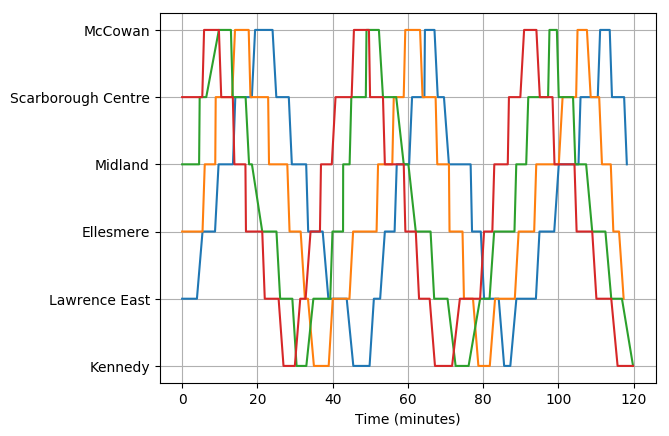
\includegraphics[width=6.0in]{Scheduler_ExpFrame4TrainsNoDelays.png}
	\caption{Scarborough line with 4 trains and no delays}\label{fig:4trainsNoDelay}
\end{figure}

\begin{figure}[tb]
	\centering
	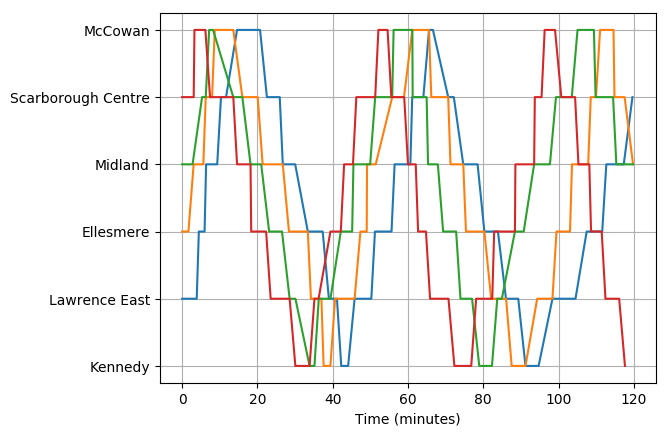
\includegraphics[width=6.0in]{Scheduler_ExpFrame4TrainsWithDelays.png}
	\caption{Scarborough line with 4 trains and delays}\label{fig:4trainsWithDelay}
\end{figure}

\begin{figure}[tb]
	\centering
	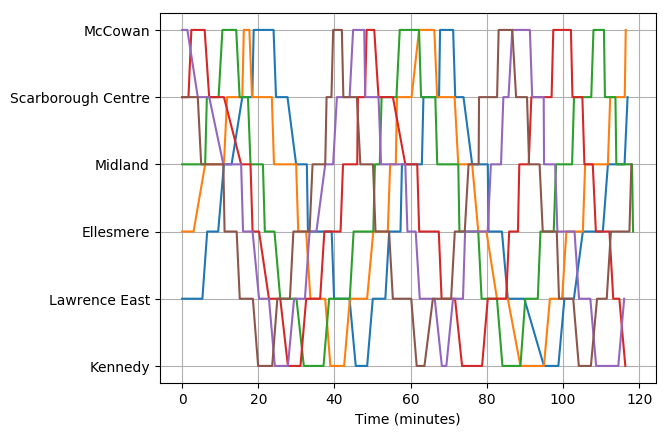
\includegraphics[width=6.0in]{Scheduler_ExpFrame6TrainsNoDelays.png}
	\caption{Scarborough line with 6 trains and no delays}\label{fig:6trainsNoDelay}
\end{figure}

\begin{figure}[tb]
	\centering
	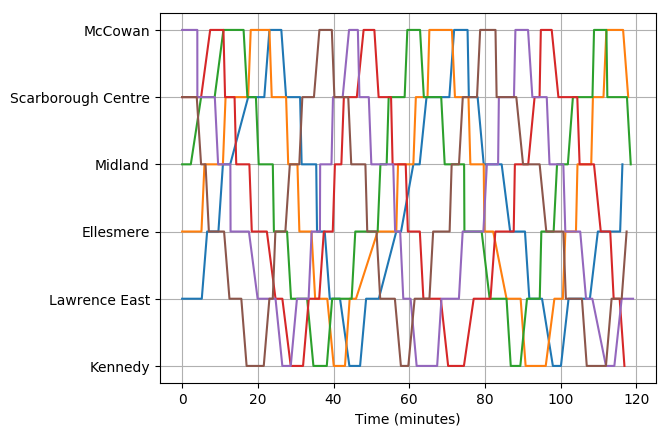
\includegraphics[width=6.0in]{Scheduler_ExpFrame6TrainsWithDelays.png}
	\caption{Scarborough line with 6 trains and delays}\label{fig:6trainsWithDelay}
\end{figure}

\begin{figure}[tb]
	\centering
	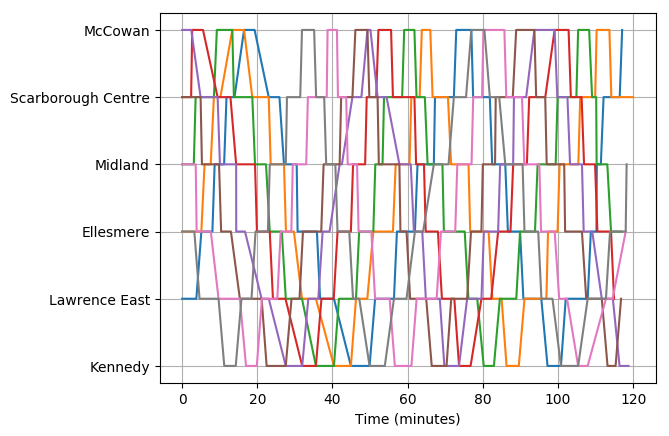
\includegraphics[width=6.0in]{Scheduler_ExpFrame8TrainsNoDelays.png}
	\caption{Scarborough line with 8 trains and no delays}\label{fig:8trainsNoDelay}
\end{figure}

\begin{figure}[tb]
	\centering
	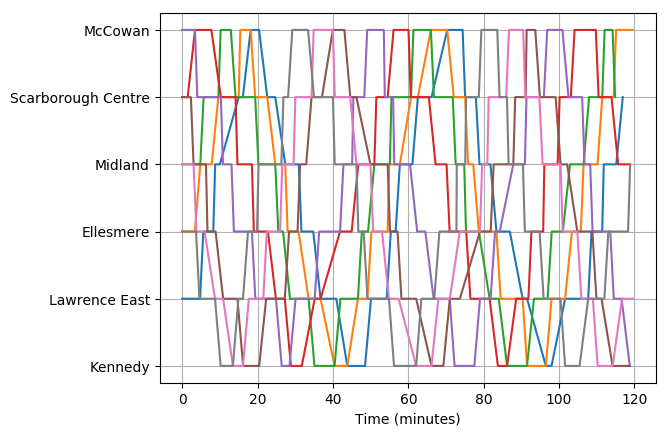
\includegraphics[width=6.0in]{Scheduler_ExpFrame8TrainsWithDelays.png}
	\caption{Scarborough line with 8 trains and delays}\label{fig:8trainsWithDelay}
\end{figure}